
\begin{figure}
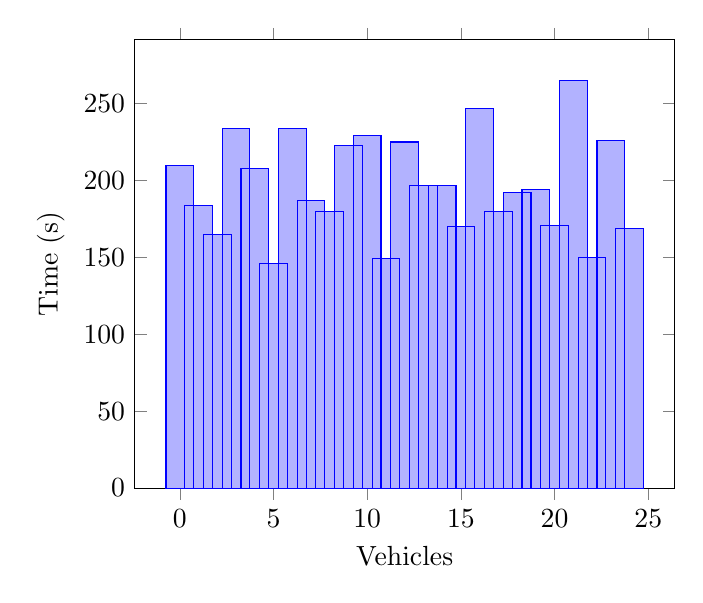
\begin{tikzpicture}
\begin{axis}[
legend style={anchor=west},
xlabel=Vehicles,
ylabel=Time (s),
ymin=0,
ybar,
]
\addplot coordinates {
(0, 210)
(1, 184)
(2, 165)
(3, 234)
(4, 208)
(5, 146)
(6, 234)
(7, 187)
(8, 180)
(9, 223)
(10, 229)
(11, 149)
(12, 225)
(13, 197)
(14, 197)
(15, 170)
(16, 247)
(17, 180)
(18, 192)
(19, 194)
(20, 171)
(21, 265)
(22, 150)
(23, 226)
(24, 169)
};

\end{axis}
\end{tikzpicture}
\label{tik:0:3_V, 3_V.-60, 4_S, 5_S, 5_S.-30, 7_S, 7_S.-25, 11_S, 11_S.-50, 13_S, 15_N, 17_S, 17_S.-60, 20_O, 21_O}
\caption{0 percent diving with GSC on route $3_V, 3_V.-60, 4_S, 5_S, 5_S.-30, 7_S, 7_S.-25, 11_S, 11_S.-50, 13_S, 15_N, 17_S, 17_S.-60, 20_O, 21_O$}
\end{figure}
